\documentclass[10pt,a4paper]{article}
\usepackage[utf8]{inputenc}
\usepackage[italian]{babel}
\usepackage{amsmath}
\usepackage{amsfonts}
\usepackage{amssymb}
\usepackage{graphicx}
\usepackage{gensymb}
\usepackage[left=2cm,right=2cm,top=2cm,bottom=2cm]{geometry}
\newcommand{\rem}[1]{[\emph{#1}]}

\author{Gruppo BN \\ Federico Belliardo, Lisa Bedini, Marco Costa}
\title{Esperienza 10: caratteristiche fisiche porte logiche}

\begin{document}
\maketitle

\section{Flip-Flop D-Latch}
Si è realizzato un circuito flip-flop di tipo D-Latch, come mostrato in figura \ref{D-Latch} utilizzando le porte NAND di due integrati. L'ingresso D che corrisponde al dato da memorizzare è stato collegato all'impulsatore realizzato con Arduino Nano (in particolare a Y1 o a Y2?), e l'Enable è collegato alla tensione positiva attraverso uno switch manuale (inserire resistenza di pull-up?)\\

\begin{figure}
\centering
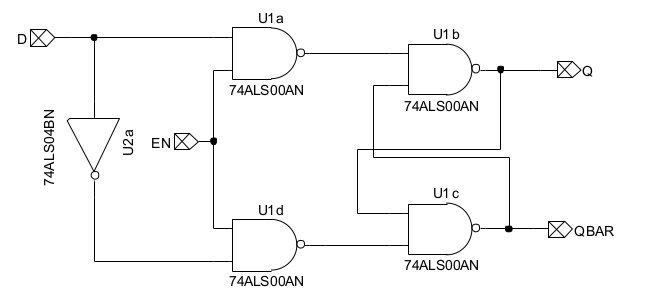
\includegraphics[scale=0.7]{flipflopDlatch.png}
\caption{Circuito utilizzato\label{fig:circuito}}
\end{figure}

In figura \ref{segue} si vede come il segnale $Q(t)$ in uscita dal flip-flop segua l'ingresso. Commutando manualmente lo switch il flip flop rimane congelato nello stato in cui si trovava prima della commutazione. Perché il valore che il flip-flop memorizza sia deterministico è necessario che la commutazione dello switch non avvenga durante gli hold-time e setup-time del latch. In figure \ref{cong1} e \ref{cong2} si vede il flip-flop congelato nei due stati. Quando il bit di enable è disattivato entrambe le uscite degli and del primo livello sono a 1 pertanto il latch è nello stato di hold.\\

Essendo il latch costruito con delle porte NAND ho una situazione di instabilità quando gli ingressi delle porte sul secondo livello sono antrambe a 0. Questo può succedere solo se gli ingressi di tutte le porte sul primo livello sono 1. IL NOT evita questa situazione.\\
L'enable è attivo alto. Cioè quando $enable = 0$ ho permanenza dello stato, infatti gli ingressi al secondo livello dei NAND sono sicuramente a 1. mentre posso avere evoluzione dello stato se il bit è: $enable = 1$.\\

Si sono misurati i tempi di ritardo sulla salita e discesa del flip-flop (quando è abilitato) essi sono risultati asimmetrici.\\

(Spiegare perché?)

\section{Divisori di frequenza}

\section{Shift register con D-Latch}







